\subsection{Vergleich der Informationsquellen}\label{subsec:vergleich}
Im Zuge des Vergleichs wurden 30 Vendors nach Unterst�tzung von RSS-Feeds, Twitter, Newsletter und Blogs analysiert. Zus�tzlich wurde das Datum des letzten Updates in Format TT.MM.JJ erfasst, das nach dem neuesten Eintrag aus den betrachteten Datenquellen zum Zeitpunkt vom 10. Mai 2017 bestimmt wird. Die Ergebnisse werden in Tabelle \ref{tab:vergleich} zusammengefasst.
\begin{table}[H] 
\centering 
\begin{tabular}{ |l|c|c|c|c|c| }
\hline
\textbf{Vendor} & \textbf{RSS} & \textbf{Twitter} & \textbf{Newsletter} & \textbf{Blogs} & \textbf{Last Update} \\ \hline
\hline
Anynines & nein & ja & ja & nein & 18.08.15 \\ \hline
App42 PaaS & nein & ja & ja & ja & 10.05.17 \\ \hline
AppFog & nein & ja & ja & ja & 10.05.17 \\ \hline
AppHarbor & nein & ja & nein & ja & 22.05.16 \\ \hline
BitNami & nein & ja & ja & ja & 10.05.17 \\ \hline
Brightbox & nein & ja & nein & ja & 25.04.17 \\ \hline
Clever Cloud & nein & ja & nein & ja & 26.04.17 \\ \hline
Cloudnode & nein & ja & nein & ja & 23.04.17 \\ \hline
CloudUnit & nein & ja & nein & nein & 10.05.17 \\ \hline
Cloudways & nein & ja & ja & ja & 10.05.17 \\ \hline
EngineYard & nein & ja & nein & ja & 29.04.17 \\ \hline
Flynn & nein & ja & ja & ja & 17.10.16 \\ \hline 
fortrabbit & nein & ja & nein & ja & 04.05.17 \\ \hline
Getup Cloud & nein & ja & nein & nein & 09.05.17 \\ \hline
Google App Engine & nein & ja & ja & ja & 10.05.17 \\ \hline
Heroku & ja & ja & ja & ja & 10.05.17 \\ \hline
Jelastic & nein & ja & ja & ja & 10.05.17 \\ \hline
Mendix & nein & ja & nein & ja & 28.04.17 \\ \hline
mOSAIC & ja & nein & nein & nein & 05.04.13 \\ \hline
OpenShift Container Platform & nein & ja & nein & ja & 22.04.17 \\ \hline
Oracle Cloud PaaS & ja & ja & nein & ja & 01.12.16 \\ \hline
OrangeScape & nein & ja & nein & ja & 05.04.17 \\ \hline
Pagoda Box & nein & ja & nein & ja & 06.05.16 \\ \hline
Platformer.com & ja & ja & nein & ja & 01.04.17 \\ \hline
SAP HANA Cloud Platform & nein & ja & nein & ja & 02.05.17 \\ \hline
Software AG Live & nein & ja & ja & ja & 10.05.17 \\ \hline
Tsuru & nein & ja & ja & ja & 12.04.17 \\ \hline
Voxoz & nein & ja & nein & nein & 08.01.17 \\ \hline
WSO2 App Cloud & nein & ja & ja & ja & 10.05.17 \\ \hline   
\end{tabular}
\caption{Vergleich von RSS, Twitter, Newsletter und Blogs} 
\label{tab:vergleich}
\end{table} 
In der Tabelle \ref{tab:vergleich} sieht man deutlich, dass Twitter die h�chste Verbreitung unter den betrachteten Quellen hat. Nur in einem Fall wird es nicht unterst�tzt, und zwar bei mOSAIC\footnote{http://www.mosaic-cloud.eu/}. Allerdings l�sst sich nach dem Datum des letzten Updates (05.04.13) sagen, dass bei mOSAIC generell nicht viel passiert. Ansonsten gilt Twitter als Favorit in Bezug auf Verbreitung, Datenformat (Kurznachrichten) und Datenzugriff (API).\\
Bei RSS sieht es leider schlecht aus. W�hrend es bei bekannten Anbietern wie Heroku hervorragend unterst�tzt wird (siehe Abbildung \ref{rss-heroku}), bieten kleinere Vendors diesen Service nicht an. Ein m�glicher Grund daf�r ist die Einfachheit von Twitter, mit dem man das Gleiche erreicht, ohne den RSS Aufwand zu haben. \\
Erstaunlicherweise sind Blogs sehr verbreitet. Meist sind Blogs f�r Publikum mit technischem Hintergrund gedacht. Aber wie bereits in Abschnitt \ref{subsec:Abgrenzung der Datenquellen} erw�hnt wurde, werden dabei die Updates in Form eines Artikels publiziert. Bez�glich der Newsletters gibt es kein klares Bild. Etwa ein Drittel der betrachteten Vendors sehen diese Option vor. Dabei muss beachtet werden, dass Newsletter fallweise zu einem Blog angeboten werden.
\begin{figure}[H] 
	\centering
	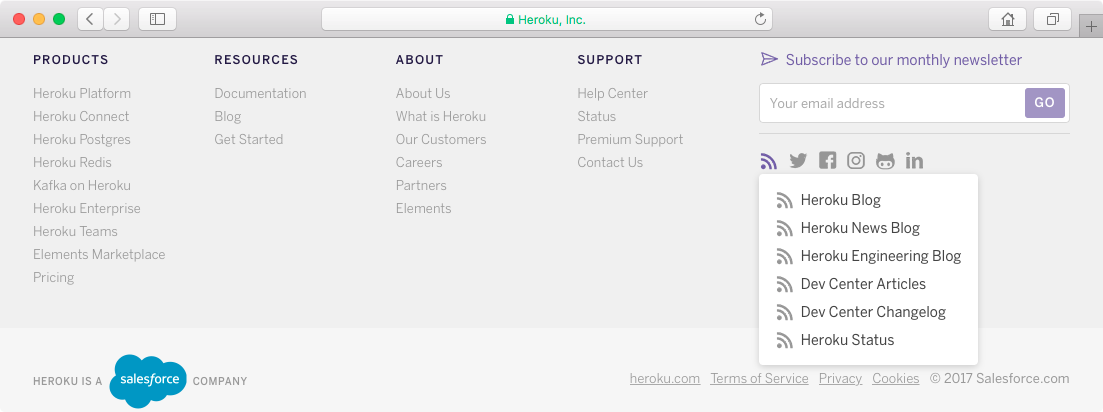
\includegraphics[width=1.0\textwidth]{images/heroku-feeds.png}
	\caption{RSS Angebot bei Heroku}
	\label{rss-heroku}
\end{figure} 